\subsection{The Abstract Syntax Tree}\label{subsec:ast}

The \emph{BookStore} concept
\footnote{For brevity,
only displaying the partial tree of the CML model defined in figure \ref{fig:store} (just for the \emph{BookStore} concept), 
but a similar tree is generated by the compiler for all other concepts.}
specified in the model of figure \ref{fig:store},
when parsed and instantiated by the CML compiler,
generates the following abstract syntax tree:

\label{fig:ast}
\begin{figure}
\centering
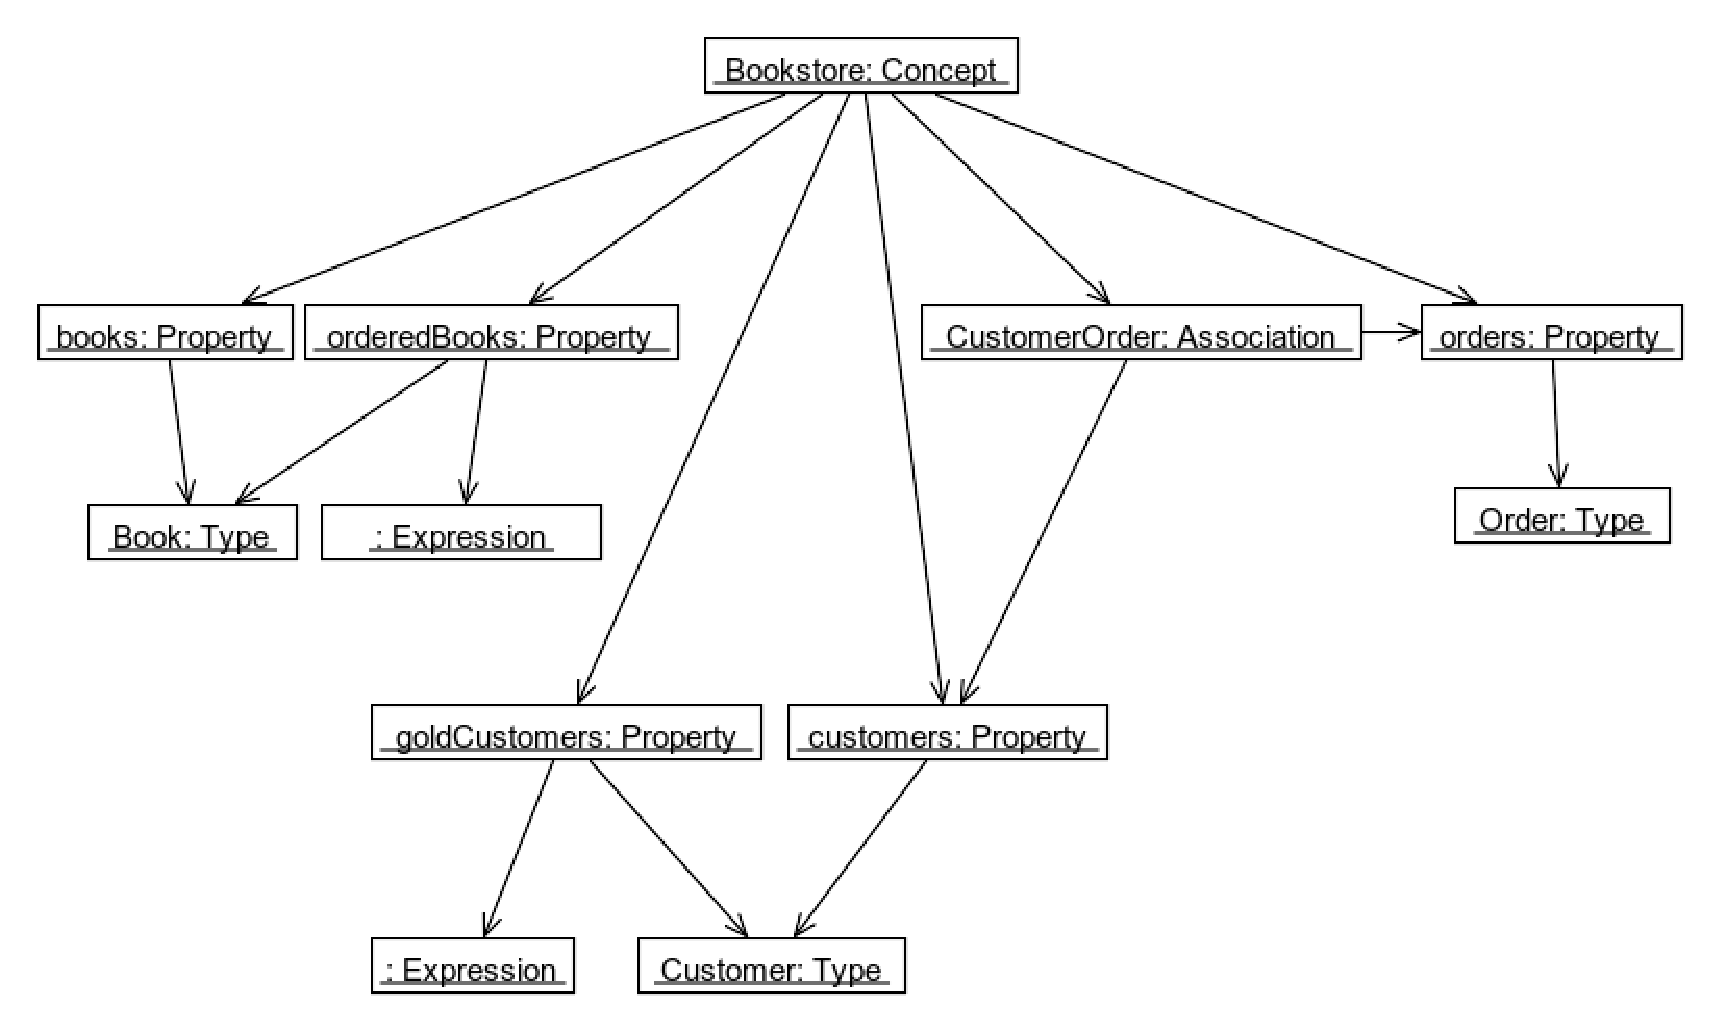
\includegraphics[width=\textwidth]{language/figure-ast}
\caption{The abstract syntax tree generated by the CML compiler after parsing the \emph{BookStore} concept.}
\end{figure}

The model above can also be represented as the following ER model:

[ER model]

The model can also be shown as the following UML class diagram:

[UML Class Diagram]
